\section{Računanje razdalje med točko in nedominiranim območjem}
\label{sec:resevanje}

V tem poglavju najprej definiramo problem računanja razdalje med točko in nedominiranim območjem in predstavimo delovanje algoritma zanj v dveh dimenzijah. Na kratko predstavimo algoritme pometanja, na katerih temelji nov algoritem. Nato predstavimo nov algoritem ARRNO za računanje razdalje do nedominiranega območja, ki rešuje problem v treh dimenzijah. Na koncu algoritem posplošimo za reševanje problemov v poljubni višji dimenziji. 


\subsection{Definicija problema in osnovne lastnosti}
Dana je množica $\P$, ki vsebuje $n$ paroma nedominiranih $D$-dimenzionalnih točk. Vse točke iz $\P$ dominirajo referenčno točko $\textbf{r} = \textbf{0}$ in so urejene padajoče po zadnji koordinati. Dana je tudi točka poizvedbe $\textbf{q} \notin N(\P)$. Izračunati želimo razdaljo med točko $\textbf{q}$ in nedominiranim območjem $N(\P)$ množice $\P$, torej
\[
d(\textbf{q}, N(\P)) = \min_{\textbf{z} \in N(\P)} d(\textbf{q}, \textbf{z}).
\]
Primer različnih poizvedbenih točk in njihovih razdalj do nedominiranega območja v dvodimenzionalnem prostoru vidimo na sliki \ref{fig:def_example}.
\begin{figure}[ht]
  \centering
  \begin{tikzpicture}
    
    % Shade the non-dominated area (above and right)
    \fill[fillcol] 
        (0,5) -- (0,4) -- (0.5,4) -- 
        (0.5,2.5) -- (1.5,2.5) -- 
        (1.5,2) -- (2,2) -- 
        (2,1.5) -- (3.5,1.5) -- 
        (3.5,0.5) -- (4,0.5) -- 
        (4,0) -- (5,0) -- (5,5) -- cycle;
    \node at (3.75,3.75) {\( N(\P) \)};


    % Draw lines from each point (downward and leftward)
    \draw (0.5,4) -- (0.5,2.5);  
    \draw (0.5,4) -- (0,4);      

    \draw (1.5,2.5) -- (1.5,2);  
    \draw (1.5,2.5) -- (0.5,2.5);

    \draw (2,2) -- (2,1.5);      
    \draw (2,2) -- (1.5,2);      

    \draw (3.5,1.5) -- (3.5,0.5);
    \draw (3.5,1.5) -- (2,1.5);  

    \draw (4,0.5) -- (4,0);      
    \draw (4,0.5) -- (3.5,0.5);  

    % Nondominated points
    \fill (0.5,4) circle (2pt) node[above right] {\( \textbf{p}^1 \)};
    \fill (1.5,2.5) circle (2pt) node[above right] {\( \textbf{p}^2 \)};
    \fill (2,2) circle (2pt) node[above right] {\( \textbf{p}^3 \)};
    \fill (3.5,1.5) circle (2pt) node[above right] {\( \textbf{p}^4 \)};
    \fill (4,0.5) circle (2pt) node[above right] {\( \textbf{p}^5 \)};

    % Additional points q1, q2, q3
    \fill[nodecol] (-0.4,4.2) circle (2pt) node[below left] {\( \textbf{q}^1 \)};
    \fill[nodecol] (0.6,1) circle (2pt) node[below left] {\( \textbf{q}^2 \)};
    \fill[nodecol] (2.5,1) circle (2pt) node[below left] {\( \textbf{q}^3 \)};
    
    % Draw lines to the nearest boundary of the non-dominated region
    \draw[nodecol] (-0.4,4.2) -- (0,4.2);  % q1 to shaded region (horizontally right)
    \draw[nodecol] (0.6, 1) -- (1.5,2);  % q2 to v (diagonal)
    \draw[nodecol] (2.5,1) -- (2.5,1.5);  % q3 to shaded region (vertically up)

    % Draw axes
    \draw[->] (0,0) -- (5,0) node[midway, below] {\( f_1 \)};
    \draw[->] (0,0) -- (0,5) node[midway, left] {\( f_2 \)};
    
    % Draw a small dot at the origin
    \fill (0,0) circle (2pt);

\end{tikzpicture}

  \caption{Tri točke poizvedbe $\textbf{q}^1$, $\textbf{q}^2$, $\textbf{q}^3$ in njihove razdalje do nedominiranega območja $N(\P)$ za $\P = \{ \textbf{p}^1, \dots, \textbf{p}^5\}$.}
  \label{fig:def_example}
\end{figure}

\begin{trditev}
\label{trditev:unija-stozcev}
Množico $N(\P)$ lahko zapišemo kot unijo stožcev, ki jih razpenja množica vpetih točk $\V(\P)$, torej
\[
N(\P) = \bigcup_{\textbf{v} \in \V(\P)} C(\textbf{v}).
\]
\end{trditev}
\begin{dokaz}
Najprej pokažemo, da velja 
\[
\forall \textbf{v} \in \V(\P): \quad C(\textbf{v}) \subseteq N(\P).
\]
Predpostavimo, da obstaja $\textbf{x} \in C(\textbf{v})$, tako da $\textbf{x} \notin N(\P)$. Torej obstaja $\textbf{p} \in \P$ da velja $\textbf{p} \ggcurly \textbf{x} \succeq \textbf{v}$. Ker pa je $\textbf{v}$ po definiciji iz $N(\P)$, neenakost $\textbf{p} \ggcurly \textbf{v}$ ne more veljati. S tem smo dobili protislovje.

Pokažimo še neenakost v drugo smer 
\[
N(\P) \subseteq \bigcup_{\textbf{v} \in \V(\P)} C(\textbf{v}).
\]
Naj bo $\textbf{x} = (x_1, x_2, \dots, x_D) \in N(\P)$. Torej za vsak $i \in \{1, \dots, D\}$ velja $x_i \geq 0$. Nadalje naj bo $v_1 = \min \{v \mid (v, x_2, \dots, x_D) \in N(\P) \}$ in $\textbf{x}^1 = (v_1, x_2, \dots, x_D)$. Tak $v_1$ gotovo obstaja, saj velja $v_1 \in \{0\} \cup \{p_1 \mid p \in \P\}$. Podobno naj bo $v_2 = \min \{v \mid (v_1, v, x_3, \dots, x_D) \in N(\P) \}$ in $\textbf{x}^2 = (v_1, v_2, x_3, \dots, x_D)$. Tako lahko definiramo vse $v_i$ in $\textbf{x}^i$ za $i \in \{1, \dots, D\}$, torej $v_i = \min \{v \mid (v_1, \dots, v_{i-1}, v, x_{i+1}, \dots, x_D) \in N(\P) \}$ ter $\textbf{x}^i = (v_1, \dots, v_i, x_{i+1}, \dots, x_D)$.

Naj bo $\textbf{v} = \textbf{x}^D = (v_1, v_2,\dots, v_D)$. Očitno je $\textbf{x} \succeq \textbf{v}$, saj za vsak $i$ velja $x_i \geq v_i$. Torej velja $\textbf{x} \in C(\textbf{v})$. Pokažimo, da velja tudi $\textbf{v} \in \V(\P)$. Predpostavimo, da to ni res in da obstaja nek $\textbf{z} \in N(\P)$, tako da velja $\textbf{v} \succ \textbf{z}$. Torej za nek $i$ velja $v_i > z_i$. Definirajmo točko $\textbf{y} = (v_1, \dots, v_{i-1}, z_i, x_{i+1}, \dots, x_D)$. Velja $\textbf{y} \in N(\P)$, saj je $\textbf{y} \succeq \textbf{z}$. Tu smo prišli do protislovja, saj smo pokazali da je $z_i < v_i$, ki je po definiciji najmanjša taka vrednost $v$ da je $(v_1, \dots, v_{i-1}, v, x_{i+1}, \dots, x_D) \in N(\P)$.
\end{dokaz}

Ilustracija stožcev $C(\textbf{v}), \textbf{v} \in \V(\P)$, za množico dvodimenzionalnih točk $\P$ je vidna na sliki~\ref{fig:cones}.
\begin{figure}[ht]
  \centering
  \begin{tikzpicture}
    % Draw axes
    \draw[->] (0,0) -- (5.5,0) node[midway, below] {\( f_1 \)};
    \draw[->] (0,0) -- (0,5) node[midway, left] {\( f_2 \)};

    % Add semi-transparent gray shaded rectangles for v_0, ..., v_5
    \fill [fill=fillcol, fill opacity=0.25] (0.7,2.5) -- (0.7,5) -- (5.5,5) -- (5.5,2.5) -- cycle;
    \fill [fill=fillcol, fill opacity=0.25] (1.5,2) -- (1.5,5) -- (5.5,5) -- (5.5,2) -- cycle;
    \fill [fill=fillcol, fill opacity=0.25] (2,1.5) -- (2,5) -- (5.5,5) -- (5.5,1.5) -- cycle;
    \fill [fill=fillcol, fill opacity=0.25] (3.5,0.5) -- (3.5,5) -- (5.5,5) -- (5.5,0.5) -- cycle;
    \fill [fill=fillcol, fill opacity=0.25] (0,4) -- (0,5) -- (5.5,5) -- (5.5,4) -- cycle;
    \fill [fill=fillcol, fill opacity=0.25] (4,0) -- (4,5) -- (5.5,5) -- (5.5,0) -- cycle;

    \fill [fill=fillcol, fill opacity=0.4] (0.7,4) -- (0.7,5) -- (5.5,5) -- (5.5,4) -- cycle;
    \fill [fill=fillcol, fill opacity=0.4] (4,0.5) -- (4,5) -- (5.5,5) -- (5.5,0.5) -- cycle;
    \fill [fill=fillcol, fill opacity=0.4] (3.5,1.5) -- (3.5,5) -- (5.5,5) -- (5.5,1.5) -- cycle;
    \fill [fill=fillcol, fill opacity=0.4] (2,2) -- (2,5) -- (5.5,5) -- (5.5,2) -- cycle;
    \fill [fill=fillcol, fill opacity=0.4] (1.5,2.5) -- (1.5,5) -- (5.5,5) -- (5.5,2.5) -- cycle;

    \fill [fill=fillcol] (5.5,5) -- (5.5,1.5) -- (4,1.5) -- (4,2) -- (3.5,2) --
                         (3.5,2.5) -- (2,2.5) -- (2,4) -- (1.5,4) -- (1.5,5) -- cycle;
    
    % Draw a small dot at the origin
    \fill (0,0) circle (2pt);


    % Draw lines from each point (downward and leftward)
    \draw (0.7,4) -- (0.7,2.5);  
    \draw (0.7,4) -- (0,4);      

    \draw (1.5,2.5) -- (1.5,2);  
    \draw (1.5,2.5) -- (0.7,2.5);

    \draw (2,2) -- (2,1.5);      
    \draw (2,2) -- (1.5,2);      

    \draw (3.5,1.5) -- (3.5,0.5);
    \draw (3.5,1.5) -- (2,1.5);  

    \draw (4,0.5) -- (4,0);      
    \draw (4,0.5) -- (3.5,0.5);  

    \fill[nodecol] (0,4) circle (2pt) node[below left] {\( \textbf{v}^0 \)};
    \fill[nodecol] (0.7,2.5) circle (2pt) node[below left] {\( \textbf{v}^1 \)};
    \fill[nodecol] (1.5,2) circle (2pt) node[below left] {\( \textbf{v}^2 \)};
    \fill[nodecol] (2,1.5) circle (2pt) node[below left] {\( \textbf{v}^3 \)};
    \fill[nodecol] (3.5,0.5) circle (2pt) node[below left] {\( \textbf{v}^4 \)};
    \fill[nodecol] (4,0) circle (2pt) node[below left] {\( \textbf{v}^5 \)};


    % Intersection points v_0, ..., v_5
    \fill[nodecol2] (0.2,4.1) node[above right] {\( C(\textbf{v}^0) \)};
    \fill[nodecol2] (0.9,2.7) node[above right] {\( C(\textbf{v}^1) \)};
    \fill[nodecol2] (1.6,2.1) node[above right] {\( C(\textbf{v}^2) \)};
    \fill[nodecol2] (2.2,1.5) node[above right] {\( C(\textbf{v}^3) \)};
    \fill[nodecol2] (3.6,0.6) node[above right] {\( C(\textbf{v}^4) \)};
    \fill[nodecol2] (4.1,0.1) node[above right] {\( C(\textbf{v}^5) \)};


    % cones
    % \fill[nodecol] (0,4) node[above right] {\( c(\textbf{v}^0) \)};
    % \fill[nodecol] (0.5,2.5) node[above right] {\( c(\textbf{v}^1) \)};
    % \fill[nodecol] (1.5,2) node[above right] {\( c(\textbf{v}^2) \)};
    % \fill[nodecol] (2,1.5) node[above right] {\( c(\textbf{v}^3) \)};
    % \fill[nodecol] (3.5,0.5) node[above right] {\( c(\textbf{v}^4) \)};
    % \fill[nodecol] (4,0) node[above right] {\( c(\textbf{v}^5) \)};

\end{tikzpicture}

  \caption{Primer stožcev $C(\textbf{v}^0), \dots, C(\textbf{v}^5)$ s svetlo rumeno barvo, katerih unija je enaka območju $N(\P)$.}
  \label{fig:cones}
\end{figure}



\subsection{Problem v dveh dimenzijah} 
\label{sec:problem_2d}
Za razumevanje intuicije algoritma v treh in več dimenzijah, si je najprej vredno ogledati kako lahko problem rešujemo v dveh dimenzijah~\cite{moarchiving}.

Dana je množica  $\P$, ki vsebuje $n$ paroma nedominiranih dvodimenzionalnih točk 
\[
\P = \{\textbf{p}^1, \dots, \textbf{p}^n\},
\]
kjer je $\textbf{p}^i = (p^i_x, p^i_y) \ggcurly \textbf{0}$. Točke so urejene po zadnji, torej $y$ koordinati. Dana je tudi poizvedbena točka $\textbf{q} = (q_x, q_y) \notin N(\P)$.

Najprej izračunamo množico vpetih točk $\V(\P) = \{\textbf{v}^0, \dots, \textbf{v}^n\}$ za množico točk $\P$. Za dve zaporedni nedominirani točki $(p^i_x, p^i_y)$ in $(p^{i+1}_x, p^{i+1}_y)$, kjer je $p^i_x < p^{i+1}_x$ in $p^i_y > p^{i+1}_y$, izračunamo njuno vpeto točko kot $\textbf{v}^i = (p^i_x, p^{i+1}_y)$. Za prvo točko $(p^1_x, p^1_y)$ izračunamo vpeto točko kot $\textbf{v}^0 = (0, p^1_y)$, za zadnjo točko pa kot $\textbf{v}^n = (p^n_x, 0)$. Primer točk iz $\P$ in njim pripadajočih vpetih točk vidimo na sliki~\ref{fig:kink_points}.
\begin{figure}[ht]
  \centering
  \begin{tikzpicture}
    % Draw axes
    \draw[->] (0,0) -- (5,0) node[midway, below] {\( f_1 \)};
    \draw[->] (0,0) -- (0,5) node[midway, left] {\( f_2 \)};
    
    % Draw a small dot at the origin
    \fill (0,0) circle (2pt);

    % Draw lines from each point (downward and leftward)
    \draw[dashed] (0.7,4) -- (0.7,2.5);  
    \draw[dashed] (0.5,4) -- (0,4);      

    \draw[dashed] (1.5,2.5) -- (1.5,2);  
    \draw[dashed] (1.5,2.5) -- (0.7,2.5);

    \draw[dashed] (2,2) -- (2,1.5);      
    \draw[dashed] (2,2) -- (1.5,2);      

    \draw[dashed] (3.5,1.5) -- (3.5,0.5);
    \draw[dashed] (3.5,1.5) -- (2,1.5);  

    \draw[dashed] (4,0.7) -- (4,0);      
    \draw[dashed] (4,0.5) -- (3.5,0.5);  
    
    % Nondominated points
    \fill (0.7,4) circle (2pt) node[above right] {\( \textbf{p}^1 \)};
    \fill (1.5,2.5) circle (2pt) node[above right] {\( \textbf{p}^2 \)};
    \fill (2,2) circle (2pt) node[above right] {\( \textbf{p}^3 \)};
    \fill (3.5,1.5) circle (2pt) node[above right] {\( \textbf{p}^4 \)};
    \fill (4,0.5) circle (2pt) node[above right] {\( \textbf{p}^5 \)};
    

    % Intersection points v_0, ..., v_5
    \fill[nodecol] (0,4) circle (2pt) node[below left] {\( \textbf{v}^0 \)};
    \fill[nodecol] (0.7,2.5) circle (2pt) node[below left] {\( \textbf{v}^1 \)};
    \fill[nodecol] (1.5,2) circle (2pt) node[below left] {\( \textbf{v}^2 \)};
    \fill[nodecol] (2,1.5) circle (2pt) node[below left] {\( \textbf{v}^3 \)};
    \fill[nodecol] (3.5,0.5) circle (2pt) node[below left] {\( \textbf{v}^4 \)};
    \fill[nodecol] (4,0) circle (2pt) node[below left] {\( \textbf{v}^5 \)};

\end{tikzpicture}

  \caption{Primer množice petih paroma nedominiranih točk $\textbf{p}^1, \dots, \textbf{p}^5$ ter njim pripadajočih vpetih točk $\textbf{v}^0, \dots, \textbf{v}^5$.}
  \label{fig:kink_points}
\end{figure}

Po trditvi~\ref{trditev:unija-stozcev} velja, da je razdalja poljubne točke poizvedbe $\textbf{q}$ do nedominiranega območja $N(\P)$ enaka minimalni razdalji točke $\textbf{q}$ do vseh stožcev
\[
d(\textbf{q}, N(\P)) = \min_{\textbf{v} \in \V(\P)} d(\textbf{q}, C(\textbf{v})),
\]
kar vidimo tudi na sliki~\ref{fig:cone_dist}.
\begin{figure}[ht]
  \centering
  \begin{tikzpicture}
    % Draw axes
    \draw[->] (0,0) -- (5,0) node[midway, below] {\( f_1 \)};
    \draw[->] (0,0) -- (0,5) node[midway, left] {\( f_2 \)};

    % Add semi-transparent gray shaded rectangles for v_0, ..., v_5
    \fill [fill=fillcol, fill opacity=0.25] (0.5,2.5) -- (0.5,5) -- (5,5) -- (5,2.5) -- cycle;
    \fill [fill=fillcol, fill opacity=0.25] (1.5,2) -- (1.5,5) -- (5,5) -- (5,2) -- cycle;
    \fill [fill=fillcol, fill opacity=0.25] (2,1.5) -- (2,5) -- (5,5) -- (5,1.5) -- cycle;
    \fill [fill=fillcol, fill opacity=0.25] (3.5,0.5) -- (3.5,5) -- (5,5) -- (5,0.5) -- cycle;
    \fill [fill=fillcol, fill opacity=0.25] (0,4) -- (0,5) -- (5,5) -- (5,4) -- cycle;
    \fill [fill=fillcol, fill opacity=0.25] (4,0) -- (4,5) -- (5,5) -- (5,0) -- cycle;

    \fill [fill=fillcol, fill opacity=0.4] (0.5,4) -- (0.5,5) -- (5,5) -- (5,4) -- cycle;
    \fill [fill=fillcol, fill opacity=0.4] (4,0.5) -- (4,5) -- (5,5) -- (5,0.5) -- cycle;
    \fill [fill=fillcol, fill opacity=0.4] (3.5,1.5) -- (3.5,5) -- (5,5) -- (5,1.5) -- cycle;
    \fill [fill=fillcol, fill opacity=0.4] (2,2) -- (2,5) -- (5,5) -- (5,2) -- cycle;
    \fill [fill=fillcol, fill opacity=0.4] (1.5,2.5) -- (1.5,5) -- (5,5) -- (5,2.5) -- cycle;

    \fill [fill=fillcol] (5,5) -- (5,1.5) -- (4,1.5) -- (4,2) -- (3.5,2) --
                         (3.5,2.5) -- (2,2.5) -- (2,4) -- (1.5,4) -- (1.5,5) -- cycle;

    
    % Draw a small dot at the origin
    \fill (0,0) circle (2pt);


    % Draw lines from each point (downward and leftward)
    \draw[dashed] (0.5,4) -- (0.5,2.5);  
    \draw[dashed] (0.5,4) -- (0,4);      

    \draw[dashed] (1.5,2.5) -- (1.5,2);  
    \draw[dashed] (1.5,2.5) -- (0.5,2.5);

    \draw[dashed] (2,2) -- (2,1.5);      
    \draw[dashed] (2,2) -- (1.5,2);      

    \draw[dashed] (3.5,1.5) -- (3.5,0.5);
    \draw[dashed] (3.5,1.5) -- (2,1.5);  

    \draw[dashed] (4,0.5) -- (4,0);      
    \draw[dashed] (4,0.5) -- (3.5,0.5);  

    % Intersection points v_0, ..., v_5
    \fill[nodecol] (0,4) circle (2pt) node[above right] {\( \textbf{v}^0 \)};
    \fill[nodecol] (0.5,2.5) circle (2pt) node[above right] {\( \textbf{v}^1 \)};
    \fill[nodecol] (1.5,2) circle (2pt) node[above right] {\( \textbf{v}^2 \)};
    \fill[nodecol] (2,1.5) circle (2pt) node[above right] {\( \textbf{v}^3 \)};
    \fill[nodecol] (3.5,0.5) circle (2pt) node[above right] {\( \textbf{v}^4 \)};
    \fill[nodecol] (4,0) circle (2pt) node[above right] {\( \textbf{v}^5 \)};


    % cones
    % \fill[nodecol] (0,4) node[above right] {\( c(\textbf{v}^0) \)};
    % \fill[nodecol] (0.5,2.5) node[above right] {\( c(\textbf{v}^1) \)};
    % \fill[nodecol] (1.5,2) node[above right] {\( c(\textbf{v}^2) \)};
    % \fill[nodecol] (2,1.5) node[above right] {\( c(\textbf{v}^3) \)};
    % \fill[nodecol] (3.5,0.5) node[above right] {\( c(\textbf{v}^4) \)};
    % \fill[nodecol] (4,0) node[above right] {\( c(\textbf{v}^5) \)};

    % Plot q point
    \fill[nodecol] (0.4,1) circle (2pt) node[below left] {\( \textbf{q} \)};

    % Connect q to the closest points of each rectangle with red lines
    \draw[nodecol, thick] (0.4,1) -- (0.4,4);     % v_0
    \draw[nodecol, thick] (0.4,1) -- (0.5,2.5); % v_1
    \draw[nodecol, thick] (0.4,1) -- (1.5,2);   % v_2
    \draw[nodecol, thick] (0.4,1) -- (2,1.5);   % v_3
    \draw[nodecol, thick] (0.4,1) -- (3.5,1); % v_4
    \draw[nodecol, thick] (0.4,1) -- (4,1);     % v_5

\end{tikzpicture}

  \caption{Primer točke $\textbf{q}$ z označenimi razdaljami do vsakega izmed šestih stožcev $C(\textbf{v}^0), \dots, C(\textbf{v}^5)$. Črti, ki označujeta razdaljo do stožcev $C(\textbf{v}^4)$ in $C(\textbf{v}^5)$, se delno prekrivata.}
  \label{fig:cone_dist}
\end{figure}

Razdaljo $d(\textbf{q}, C(\textbf{v}))$ pa izračunamo kot
\[
d(\textbf{q}, C(\textbf{v})) = \sqrt{\max \{0, v_x - q_x\}^2 + \max \{0, v_y - q_y\}^2}. 
\]

Algoritem~\ref{alg:2d} prikazuje psevdokodo algoritma za računanje razdalje med točko in nedominiranim območjem v dveh dimenzijah. Kot smo pojasnili, najprej izračunamo vpete točke $\V(\P)$, nato pa poiščemo minimalno razdaljo med točko $\textbf{q}$ in stožci $C(\textbf{v})$, ki jih definirajo vpete točke $\textbf{v} \in \V(\P)$.
\begin{algorithm}[ht]
\caption{Algoritem ARRNO za računanje razdalje med točko in nedominiranim območjem.}
\begin{algorithmic}
\Function{ARRNO}{$\P, \textbf{q}$}
\State $\V(\P) \gets$ \Call{Vpete točke}{$\P$}
\State{$d_{\min} \gets \infty$}
\ForAll{$\textbf{v} \in \V(\P)$}
    \State $d \gets$ \Call{Razdalja do stožca}{$\textbf{q}, \textbf{v}$}
    \If{$d < d_{\min}$}
        \State{$d_{\min} \gets d$}
    \EndIf
\EndFor
\State \Return $d_{\min}$
\EndFunction
\end{algorithmic}
\label{alg:2d}
\end{algorithm}


\subsection{Problem v treh dimenzijah}
Podobno kot pri problemu v dveh dimenzijah, je pri problemu v treh dimenzijah dana množica paroma nedominiranih točk 
\[
\P = \{\textbf{p}^1, \dots, \textbf{p}^n\},
\]
kjer je $\textbf{p}^i = (p^i_x, p^i_y, p^i_z) \ggcurly \textbf{0}$. Točke so urejene padajoče po tretji koordinati. Prav tako je dana točka $\textbf{q} = (q_x, q_y, q_z) \notin N(\P)$.

Na sliki~\ref{fig:points3d} vidimo primer množice točk $\P$ in območja, ki ga točke dominirajo v treh dimenzijah. Zanima nas torej razdalja med točko $\textbf{q}$, ki se nahaja znotraj tega telesa, in površjem telesa. 
\begin{figure}[htb]
  \centering
  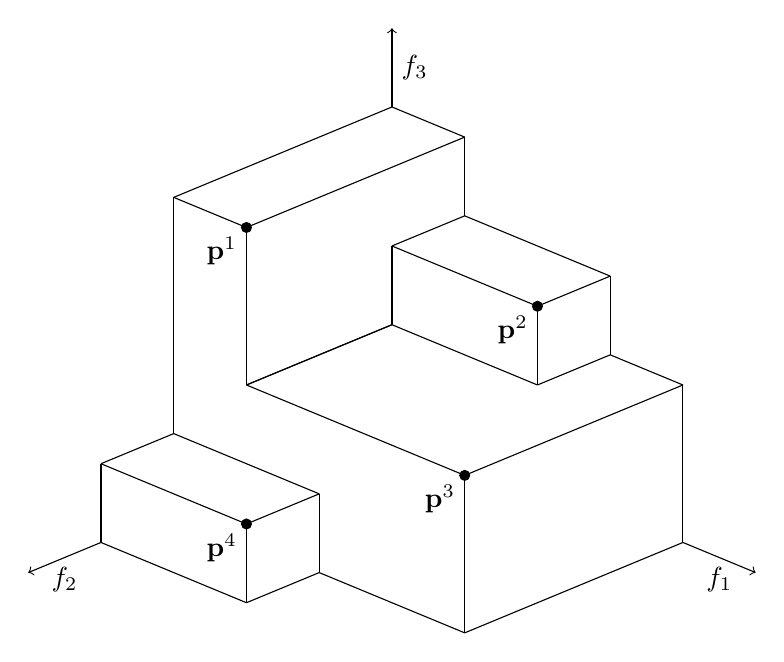
\begin{tikzpicture}
    % lines:
    \draw (-1.8478,2.4693) -- (-2.7716,2.8519);
    \draw (-2.7716,2.8519) -- (0.0,4.0);
    \draw (-2.7716,2.8519) -- (-2.7716,-0.1481);
    \draw (-1.8478,2.4693) -- (0.9239,3.6173);
    \draw (0.9239,3.6173) -- (0.0,4.0);
    \draw (0.9239,3.6173) -- (0.9239,2.6173);
    \draw (-1.8478,2.4693) -- (-1.8478,0.4693);
    \draw (-1.8478,0.4693) -- (0.0,1.2346);
    \draw (1.8478,1.4693) -- (0.0,2.2346);
    \draw (0.0,2.2346) -- (0.9239,2.6173);
    \draw (0.0,2.2346) -- (0.0,1.2346);
    \draw (1.8478,1.4693) -- (2.7716,1.8519);
    \draw (2.7716,1.8519) -- (0.9239,2.6173);
    \draw (2.7716,1.8519) -- (2.7716,0.8519);
    \draw (1.8478,1.4693) -- (1.8478,0.4693);
    \draw (1.8478,0.4693) -- (0.0,1.2346);
    \draw (1.8478,0.4693) -- (2.7716,0.8519);
    \draw (0.9239,-0.6788) -- (-1.8478,0.4693);
    \draw (-1.8478,0.4693) -- (0.0,1.2346);
    \draw (0.9239,-0.6788) -- (3.6955,0.4693);
    \draw (3.6955,0.4693) -- (2.7716,0.8519);
    \draw (3.6955,0.4693) -- (3.6955,-1.5307);
    \draw (0.9239,-0.6788) -- (0.9239,-2.6788);
    \draw (0.9239,-2.6788) -- (-0.9239,-1.9134);
    \draw (0.9239,-2.6788) -- (3.6955,-1.5307);
    \draw (-1.8478,-1.2961) -- (-3.6955,-0.5307);
    \draw (-3.6955,-0.5307) -- (-2.7716,-0.1481);
    \draw (-3.6955,-0.5307) -- (-3.6955,-1.5307);
    \draw (-1.8478,-1.2961) -- (-0.9239,-0.9134);
    \draw (-0.9239,-0.9134) -- (-2.7716,-0.1481);
    \draw (-0.9239,-0.9134) -- (-0.9239,-1.9134);
    \draw (-1.8478,-1.2961) -- (-1.8478,-2.2961);
    \draw (-1.8478,-2.2961) -- (-3.6955,-1.5307);
    \draw (-1.8478,-2.2961) -- (-0.9239,-1.9134);
    % points:
    \fill[black] (-1.8477590650225733,2.4692662705396407) circle (2pt) node[below left] {\( \textbf{p}^{1} \)};
    \fill[black] (1.8477590650225733,1.4692662705396409) circle (2pt) node[below left] {\( \textbf{p}^{2} \)};
    \fill[black] (0.923879532511287,-0.6787840265556282) circle (2pt) node[below left] {\( \textbf{p}^{3} \)};
    \fill[black] (-1.8477590650225735,-1.2961005941905386) circle (2pt) node[below left] {\( \textbf{p}^{4} \)};
    % axes:
    \draw[->] (3.6955,-1.5307) -- (4.6194,-1.9134) node[midway, below] {\( f_1 \)};
    \draw[->] (-3.6955,-1.5307) -- (-4.6194,-1.9134) node[midway, below] {\( f_2 \)};
    \draw[->] (0.0,4.0) -- (0.0,5.0) node[midway, right] {\( f_3 \)};
\end{tikzpicture}
  \caption{Točke $\textbf{p}^1$, $\textbf{p}^2$, $\textbf{p}^3$ in $\textbf{p}^4$ definirajo dominirano območje v treh dimenzijah.}
  \label{fig:points3d}
\end{figure}

Po trditvi~\ref{trditev:unija-stozcev} velja, da se množica nedominiranih točk zapiše kot unija tridimenzionalnih stožcev, ki izhajajo iz točk $\V(\P)$, kot vidimo na sliki~\ref{fig:points3dkink}. 
\begin{figure}[htb]
  \centering
  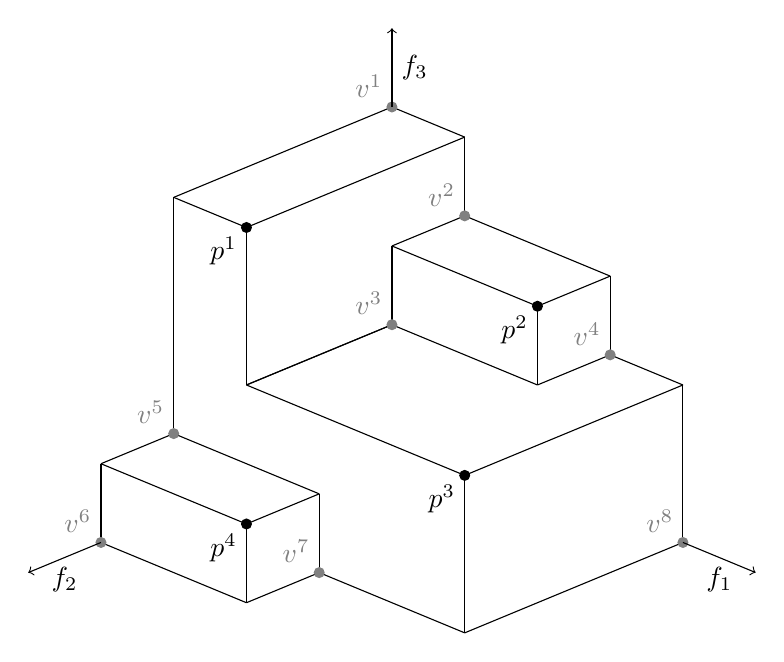
\begin{tikzpicture}
    % lines:
    \draw (-1.8478,2.4693) -- (-2.7716,2.8519);
    \draw (-2.7716,2.8519) -- (0.0,4.0);
    \draw (-2.7716,2.8519) -- (-2.7716,-0.1481);
    \draw (-1.8478,2.4693) -- (0.9239,3.6173);
    \draw (0.9239,3.6173) -- (0.0,4.0);
    \draw (0.9239,3.6173) -- (0.9239,2.6173);
    \draw (-1.8478,2.4693) -- (-1.8478,0.4693);
    \draw (-1.8478,0.4693) -- (0.0,1.2346);
    \draw (1.8478,1.4693) -- (0.0,2.2346);
    \draw (0.0,2.2346) -- (0.9239,2.6173);
    \draw (0.0,2.2346) -- (0.0,1.2346);
    \draw (1.8478,1.4693) -- (2.7716,1.8519);
    \draw (2.7716,1.8519) -- (0.9239,2.6173);
    \draw (2.7716,1.8519) -- (2.7716,0.8519);
    \draw (1.8478,1.4693) -- (1.8478,0.4693);
    \draw (1.8478,0.4693) -- (0.0,1.2346);
    \draw (1.8478,0.4693) -- (2.7716,0.8519);
    \draw (0.9239,-0.6788) -- (-1.8478,0.4693);
    \draw (-1.8478,0.4693) -- (0.0,1.2346);
    \draw (0.9239,-0.6788) -- (3.6955,0.4693);
    \draw (3.6955,0.4693) -- (2.7716,0.8519);
    \draw (3.6955,0.4693) -- (3.6955,-1.5307);
    \draw (0.9239,-0.6788) -- (0.9239,-2.6788);
    \draw (0.9239,-2.6788) -- (-0.9239,-1.9134);
    \draw (0.9239,-2.6788) -- (3.6955,-1.5307);
    \draw (-1.8478,-1.2961) -- (-3.6955,-0.5307);
    \draw (-3.6955,-0.5307) -- (-2.7716,-0.1481);
    \draw (-3.6955,-0.5307) -- (-3.6955,-1.5307);
    \draw (-1.8478,-1.2961) -- (-0.9239,-0.9134);
    \draw (-0.9239,-0.9134) -- (-2.7716,-0.1481);
    \draw (-0.9239,-0.9134) -- (-0.9239,-1.9134);
    \draw (-1.8478,-1.2961) -- (-1.8478,-2.2961);
    \draw (-1.8478,-2.2961) -- (-3.6955,-1.5307);
    \draw (-1.8478,-2.2961) -- (-0.9239,-1.9134);
    % points:
    \fill[black] (-1.8477590650225733,2.4692662705396407) circle (2pt) node[below left] {\( p^{1} \)};
    \fill[black] (1.8477590650225733,1.4692662705396409) circle (2pt) node[below left] {\( p^{2} \)};
    \fill[black] (0.923879532511287,-0.6787840265556282) circle (2pt) node[below left] {\( p^{3} \)};
    \fill[black] (-1.8477590650225735,-1.2961005941905386) circle (2pt) node[below left] {\( p^{4} \)};
    % kink points:
    \fill[gray] (0.0,4.0) circle (2pt) node[above left] {\( v^{1} \)};
    \fill[gray] (0.9238795325112867,2.6173165676349104) circle (2pt) node[above left] {\( v^{2} \)};
    \fill[gray] (0.0,1.2346331352698203) circle (2pt) node[above left] {\( v^{3} \)};
    \fill[gray] (2.77163859753386,0.8519497029047307) circle (2pt) node[above left] {\( v^{4} \)};
    \fill[gray] (-2.77163859753386,-0.1480502970952693) circle (2pt) node[above left] {\( v^{5} \)};
    \fill[gray] (-3.695518130045147,-1.5307337294603591) circle (2pt) node[above left] {\( v^{6} \)};
    \fill[gray] (-0.9238795325112865,-1.913417161825449) circle (2pt) node[above left] {\( v^{7} \)};
    \fill[gray] (3.695518130045147,-1.5307337294603591) circle (2pt) node[above left] {\( v^{8} \)};
    % axes:
    \draw[->] (3.6955,-1.5307) -- (4.6194,-1.9134) node[midway, below] {\( f_1 \)};
    \draw[->] (-3.6955,-1.5307) -- (-4.6194,-1.9134) node[midway, below] {\( f_2 \)};
    \draw[->] (0.0,4.0) -- (0.0,5.0) node[midway, right] {\( f_3 \)};
\end{tikzpicture}
  \caption{Množica vpetih točk $\V(\P) = \{\textbf{v}^0, \dots, \textbf{v}^7\}$ za dano množico štirih nedominiranih točk $\P$.}
  \label{fig:points3dkink}
\end{figure}

Razdaljo med točko in tridimenzionalnim stožcem enostavno razširimo na tri dimenzije
\[
d(\textbf{q}, C(\textbf{v})) = \sqrt{\max \{0, v_x - q_x\}^2 + \max \{0, v_y - q_y\}^2 + \max \{0, v_z - q_z\}^2}. 
\]
Torej lahko uporabimo Algoritem~\ref{alg:2d} in se iskanje razdalje točke do nedominiranega prostora prevede na problem iskanja množice vpetih točk $\V(\P)$. Vendar pa je iskanje množice $\V(\P)$ v treh dimenzijah precej bolj zapleteno kot v dveh dimenzijah, kjer lahko za vsak par sosednjih točk enostavno izračunamo njuno vpeto točko. Vidimo sicer nekatere podrobnosti, točka $\textbf{v}^2 = (p^1_x, p^2_y, p^3_z)$ iz slike~\ref{fig:points3dkink} dobi po eno koordinato od vsake izmed njej ``sosednjih'' točk iz $\P$, vendar pojem sosednosti v treh dimenzijah ni jasno definiran. Prav tako bi se radi izognili kubični časovni zahtevnosti preverjanja vsake trojice točk $(\textbf{p}^i, \textbf{p}^j, \textbf{p}^k)$ in računanja njihove vpete točke, če ta sploh obstaja. Zato za iskanje vpetih točk uporabimo algoritem pometanja.  

\subsubsection{Algoritmi pometanja}
Algoritmi pometanja so pomemben pristop v računski geometriji, ki omogoča sistematično reševanje različnih geometrijskih problemov, kot so učinkovito iskanje presečišč daljic, določanje konveksne ovojnice točk, Delaunayeva triangulacija in številni drugi~\cite{BergCheongKreveldOvermars2008}. 
Osnovna ideja, skupna vsem algoritmom, je sistematična obdelava objektov v neki smeri premikanja oziroma pometanja ter sprotno posodabljanje stanja. Ko premica, ravnina (ali kak drug objekt s katerim pometamo) doseže novo točko, se stanje ustrezno posodobi. 
Ko prostor pometamo s hiperravnino, pri tem na vsakem koraku fiksiramo koordinato pometanja. S tem problem razdelimo na več podproblemov manjše dimenzije, kar olajša njegovo reševanje. Takemu pristopu pravimo pometanje dimenzije (angl. dimension sweep).

Pri analizi časovne zahtevnosti algoritmov pometanja je ključno določiti največje število posodobitev stanja ter časovno zahtevnost posamezne posodobitve. Pohitritve navadno dosežemo s podatkovnimi strukturami za stanje, ki podpirajo posodobitve v čim hitrejšem času, največkrat konstantnem oziroma logaritemskem, glede na velikost stanja. 

\subsubsection{Iskanje vpetih točk v treh dimenzijah} \label{sec:vpete_tocke3d}
Vpete točke iščemo z algoritmom pometanja. Pometamo z navidezno ravnino vzporedno z ravnino $xy$ od $z=\infty$ proti $z=0$ ter obravnavamo dogodke, ko se ravnina dotakne kakšne izmed točk $\textbf{p}^i$. Stanje predstavimo z dvema množicama $\sp, \sv \subset \R^2$. Množica $\sp$ vsebuje množico paroma nedominiranih projekcij že obiskanih točk na ravnino $xy$, množica $\sv$ pa vsebuje vpete točke te množice, torej $\sv = \V(\sp)$. Projekcijo točke $\textbf{p} = (p_x, p_y, p_z)$ oziroma $\textbf{v} = (v_x, v_y, v_z)$ na ravnino $xy$ označimo s $\overline{\textbf{p}} = (p_x, p_y)$ oziroma $\overline{\textbf{v}} = (v_x, v_y)$. Za pravilno obravnavo primera, ko ima več točk iz $\P$ enako $z$ koordinato, definiramo še zgoščevalno funkcijo $h$. Pri dodajanju nove točke $\overline{\textbf{v}}$ v stanje $\sv$ kot ključ v zgoščevalno funkcijo $h$ dodamo točko $\overline{\textbf{v}}$ kot vrednost pa tisto vrednost $z$, pri kateri je bila točka $\overline{\textbf{v}}$ dodana v stanje $\sv$. Takšna struktura za vsako točko $\overline{\textbf{v}}$ omogoča tudi možnost hitrega preverjanja ali je točka že bila dodana v $\sv$.

Stanje $\sp$ na začetku inicializiramo prazno, stanje $\sv$ pa vsebuje točko $\overline{\textbf{v}}^0=(0, 0)$. Prav tako inicializirimo prazno množico $\V(\P)$, kamor bomo tekom algoritma dodajali že izračunane vpete točke. Nato začnemo obravnavo točk. Na $i$-tem koraku, torej ko obravnavamo točko $\textbf{p}^i$, naredimo sledeče:
\begin{enumerate}
    \item Iz stanja $\sv$ odstranimo množico dvodimenzionalnih točk $\overline{\V}_i$, ki jih točka $\overline{\textbf{p}}^i$ strogo dominira. 
    \item V izhodno množico $\V(\P)$ dodamo množico točk $\{(\overline{v}_x, \overline{v}_y, p^i_z) \mid (\overline{v}_x, \overline{v}_y) \in \overline{\V}_i \land h((\overline{v}_x, \overline{v}_y)) \neq p^i_z \}$. Točk za katere velja $h((\overline{v}_x, \overline{v}_y)) = p^i_z$ v $\V(\P)$ ne dodamo, saj ne ustrezajo definiciji vpetih točk. 
    \item Točko $\overline{\textbf{p}}^i$ dodamo v stanje $\sp$, iz katerega odstranimo vse točke, ki jih dominira. 
    \item Stanju $\sv$ dodamo vpeti točki, ki sta nastali ob dodajanju $\overline{\textbf{p}}^i$ v stanje $\sp$. Za vsako izmed točk, nastavimo vrednost funkcije $h$ na $p^i_z$.
\end{enumerate}
Te korake ponovimo za vsako točko $\textbf{p}^i \in \P$, po padajočem vrstnem redu zadnje koordinate. Po zadnjem koraku dodamo vsem točkam $\overline{\textbf{v}}$, ki so še vedno v stanju $\sv$ tretjo koordinato 0 ter jih dodamo v izhodno množico vpetih točk $\V(\P)$. Podrobno psevdokodo predstavimo v algoritmu~\ref{alg:vpete_tocke_3d}. Funkcija \Call{Odstrani dominirane}{$\sv, \overline{\textbf{p}}$} odstrani in vrne točke iz $\sv$, ki jih točka $\overline{\textbf{p}}$ dominira, funkcija \Call{Dodaj}{$\sp, \overline{\textbf{p}}$} v stanje $\sp$ doda točko $\overline{\textbf{p}}$ ter pri tem odstrani dominirane točke, funkcija \Call{Novi vpeti točki}{$\sp, \overline{\textbf{p}}$} pa vrne vpeti točki, ki nastaneta z dodajanjem $\overline{\textbf{p}}$ v $\sp$. 

Intuitivno si lahko delovanje algoritma predstavljamo kot zaporedno rezanje telesa iz slike~\ref{fig:points3dkink} na različnih višinah $z$, kjer stanji $\sp$ in $\sv$ hranita obliko trenutnega prereza. 

\begin{algorithm}[ht]
\caption{Računanje vpetih točk v treh dimenzijah}
\begin{algorithmic}[1]
\Function{Vpete točke 3D}{$\P$}
\State{$\V(\P) \gets \{\}$}
\State{$\sp \gets \{\}$}
\State{$\sv \gets \{(0, 0)\}$}
\State{$h((0, 0)) \gets \infty$}
\For{$\textbf{p} = \textbf{p}^1, \dots, \textbf{p}^n$} \Comment{Točke so urejene po $z$ koordinati}
    \State $\sv, \overline{\V} \gets$ \Call{Odstrani dominirane}{$\sv, \overline{\textbf{p}}$}
    \ForAll{$\overline{\textbf{v}} \in \overline{\V}$}
        \If{$\overline{\textbf{p}} \ggcurly \overline{\textbf{v}} \land p_z < h(\overline{v})$}
            \State $\V(\P) \gets \V(\P) \cup \{(\overline{v_x}, \overline{v_y}, p_z)\}$
        \EndIf
    \EndFor

    \State $\sp \gets$ \Call{Dodaj}{$\sp, \overline{\textbf{p}}$}

    \State $\{\widetilde{\textbf{v}_1}, \widetilde{\textbf{v}_2}\} \gets$ \Call{Novi vpeti točki}{$\sp, \overline{\textbf{p}}$}
        \ForAll{$\textbf{v} \in \{\widetilde{\textbf{v}_1}, \widetilde{\textbf{v}_2}\}$}
        \If{$\textbf{v} \notin h$}
            \State $h(\textbf{v}) \gets p_z$
            \State $\sv \gets \sv \cup \{ \textbf{v} \}$
        \EndIf
    \EndFor 
\EndFor
\ForAll{$\textbf{v} \in \sv$}
    \State $\V(\P) \gets (v_x, v_y, 0)$
\EndFor
\State \Return $\V(\P)$
\EndFunction
\end{algorithmic}
\label{alg:vpete_tocke_3d}
\end{algorithm}

\paragraph{Primer delovanja}
Oglejmo si delovanje algoritma na primeru točk, ki smo jih videli že na sliki~\ref{fig:points3d}, torej $\textbf{p}^1 = (1, 3, 4)$, $\textbf{p}^2 = (3, 1, 3)$, $\textbf{p}^3 = (4, 3, 2)$ in $\textbf{p}^4 = (2, 4, 1)$. Na sliki \ref{fig:sweep} poleg vsakega koraka dodamo vizualizacijo, ki prikazuje stanji $\sp$ in $\sv$ po obravnavi dogodka.

\begin{enumerate}[label=\alph*)]
    \item Stanje $\sp$ inicializiramo prazno, stanje $\sv$ pa na začetku vsebuje točko $\overline{\textbf{v}}^0 = (0, 0)$, kjer je $h(\overline{\textbf{v}}^0) = \infty$.

    \begin{figure}[p]
    \centering
    \begin{subfigure}{0.45\textwidth}
        \centering
        \begin{tikzpicture}
    % lines:
    
    % points:
    
    % kink points:
    \fill[nodecol2] (0,0) circle (2pt) node[above left] {\( \overline{\textbf{v}}^{0} \)};
    
    % removed kink points
    
    % axes:
    \draw[->] (0,0) -- (5,0) node[midway, below] {\( f_1 \)};
    \draw[->] (0,0) -- (0,5) node[midway, left] {\( f_2 \)};
\end{tikzpicture}
        \caption{Stanji pred obravnavo točke $\textbf{p}^1$: \\
        $\sp = \{\}$, $\sv = \{\overline{\textbf{v}}^0\}$.}
        \label{fig:sweep_a}
    \end{subfigure}
    \hfill
    \begin{subfigure}{0.45\textwidth}
        \centering
        \begin{tikzpicture}
    % lines:
    \draw (0,3) -- (1,3);
    \draw (1,3) -- (1,0);
    
    % points:
    \fill[black] (1,3) circle (2pt) node[above right] {\( \overline{\textbf{p}}^{1} \)};
    
    % kink points:
    \fill[nodecol2] (0,3) circle (2pt) node[above left] {\( \overline{\textbf{v}}^{1} \)};
    \fill[nodecol2] (1,0) circle (2pt) node[above left] {\( \overline{\textbf{v}}^{2} \)};
    
    % removed kink points
    \fill[gray] (0,0) circle (2pt) node[above left] {\( \overline{\textbf{v}}^{0} \)};
    
    % axes:
    \draw[->] (0,0) -- (5,0) node[midway, below] {\( f_1 \)};
    \draw[->] (0,0) -- (0,5) node[midway, left] {\( f_2 \)};
\end{tikzpicture}
        \caption{Stanji po obravnavi točke $\textbf{p}^1$: \\ 
        $\sp = \{\overline{\textbf{p}}^1\}$, $\sv = \{\overline{\textbf{v}}^1, \overline{\textbf{v}}^2\}$.}
        \label{fig:sweep_b}
    \end{subfigure}

    \vspace{0.5cm}

    \begin{subfigure}{0.45\textwidth}
        \centering
        \begin{tikzpicture}
    % lines:
    \draw (0,3) -- (1,3);
    \draw (1,3) -- (1,1);
    \draw (1,1) -- (3,1);
    \draw (3,1) -- (3,0);

    % removed lines:
    \draw[dashed, gray] (1, 0) -- (1,1);
    
    % points:
    \fill[black] (1,3) circle (2pt) node[above right] {\( \overline{\textbf{p}}^{1} \)};
    \fill[black] (3,1) circle (2pt) node[above right] {\( \overline{\textbf{p}}^{2} \)};
    % kink points:
    \fill[nodecol2] (0,3) circle (2pt) node[above left] {\( \overline{\textbf{v}}^{1} \)};
    \fill[nodecol2] (1,1) circle (2pt) node[above left] {\( \overline{\textbf{v}}^{3} \)};
    \fill[nodecol2] (3,0) circle (2pt) node[above left] {\( \overline{\textbf{v}}^{4} \)};

    % removed kink points
    \fill[gray] (1,0) circle (2pt) node[above left] {\( \overline{\textbf{v}}^{2} \)};

    % axes:
    \draw[->] (0,0) -- (5,0) node[midway, below] {\( f_1 \)};
    \draw[->] (0,0) -- (0,5) node[midway, left] {\( f_2 \)};
\end{tikzpicture}
        \caption{Stanji po obravnavi točke $\textbf{p}^2$: \\ $\sp = \{\overline{\textbf{p}}^1, \overline{\textbf{p}}^2\}$, $\sv = \{\overline{\textbf{v}}^1, \overline{\textbf{v}}^3, \overline{\textbf{v}}^4\}$.}
    \end{subfigure}
    \hfill
    \begin{subfigure}{0.45\textwidth}
        \centering
        \begin{tikzpicture}
    % lines:
    \draw (0,3) -- (4,3);
    \draw (4,3) -- (4,0);

    % removed lines:
    \draw[dashed, gray] (1, 3) -- (1,1);
    \draw[dashed, gray] (3, 1) -- (1,1);
    \draw[dashed, gray] (3, 1) -- (3,0);
    
    % points:
    \fill[black] (4,3) circle (2pt) node[above right] {\( \overline{\textbf{p}}^{3} \)};
    
    % kink points:
    \fill[nodecol2] (0,3) circle (2pt) node[above left] {\( \overline{\textbf{v}}^{1} \)};
    \fill[nodecol2] (4,0) circle (2pt) node[above left] {\( \overline{\textbf{v}}^{5} \)};

    % removed kink points
    \fill[gray] (1,1) circle (2pt) node[above left] {\( \overline{\textbf{v}}^{3} \)};
    \fill[gray] (3,0) circle (2pt) node[above left] {\( \overline{\textbf{v}}^{4} \)};
    
    % axes:
    \draw[->] (0,0) -- (5,0) node[midway, below] {\( f_1 \)};
    \draw[->] (0,0) -- (0,5) node[midway, left] {\( f_2 \)};
\end{tikzpicture}
        \caption{Stanji po obravnavi točke $\textbf{p}^3$: \\  $\sp = \{\overline{\textbf{p}}^3\}$, $\sv = \{\overline{\textbf{v}}^1, \overline{\textbf{v}}^5\}$.}
    \end{subfigure}

    \vspace{0.5cm}

    \begin{subfigure}{0.45\textwidth}
        \centering
        \begin{tikzpicture}
    % lines:
    \draw (0,4) -- (2,4);
    \draw (2,4) -- (2,3);
    \draw (2,3) -- (4,3);
    \draw (4,3) -- (4,0);

    % removed lines:
    \draw[dashed, gray] (2,3) -- (0,3);

    % points:
    \fill[black] (2,4) circle (2pt) node[above right] {\( \overline{\textbf{p}}^{4} \)};
    \fill[black] (4,3) circle (2pt) node[above right] {\( \overline{\textbf{p}}^{3} \)};
    
    % kink points:
    \fill[nodecol2] (0,4) circle (2pt) node[above left] {\( \overline{\textbf{v}}^{6} \)};
    \fill[nodecol2] (2,3) circle (2pt) node[above left] {\( \overline{\textbf{v}}^{7} \)};
    \fill[nodecol2] (4,0) circle (2pt) node[above left] {\( \overline{\textbf{v}}^{5} \)};

    % removed kink points
    \fill[gray] (0,3) circle (2pt) node[above left] {\( \overline{\textbf{v}}^{1} \)};
    
    % axes:
    \draw[->] (0,0) -- (5,0) node[midway, below] {\( f_1 \)};
    \draw[->] (0,0) -- (0,5) node[midway, left] {\( f_2 \)};
\end{tikzpicture}
        \caption{Stanji po obravnavi točke $\textbf{p}^4$: \\ $\sp = \{\overline{\textbf{p}}^3, \overline{\textbf{p}}^4\}$, $\sv = \{\overline{\textbf{v}}^5, \overline{\textbf{v}}^6, \overline{\textbf{v}}^7\}$.}
    \end{subfigure}
    \hfill
    \begin{subfigure}{0.45\textwidth}
        \centering
        \begin{tikzpicture}
    % lines:
    
    % removed lines:
    \draw[dashed, gray] (0,4) -- (2,4);
    \draw[dashed, gray] (2,4) -- (2,3);
    \draw[dashed, gray] (2,3) -- (4,3);
    \draw[dashed, gray] (4,3) -- (4,0);

    % points:
    
    % kink points:
    
    % removed kink points
    \fill[gray] (0,4) circle (2pt) node[above left] {\( \overline{\textbf{v}}^{6} \)};
    \fill[gray] (2,3) circle (2pt) node[above left] {\( \overline{\textbf{v}}^{7} \)};
    \fill[gray] (4,0) circle (2pt) node[above left] {\( \overline{\textbf{v}}^{5} \)};

    
    % axes:
    \draw[->] (0,0) -- (5,0) node[midway, below] {\( f_1 \)};
    \draw[->] (0,0) -- (0,5) node[midway, left] {\( f_2 \)};
\end{tikzpicture}
        \caption{Iz stanja $\sv$ odstranimo preostale točke $\overline{\textbf{v}}^5$, $ \overline{\textbf{v}}^6$ in $\overline{\textbf{v}}^7$.}
    \end{subfigure}

    \caption{Slike prikazujejo stanje $\sp$ (črna barva), točke v stanju $\sv$ (rumena barva) ter odstranjene točke iz $\sv$ v trenutnem koraku (siva barva) na vsakem koraku algoritma.}
    \label{fig:sweep}
\end{figure}


    
    \item Na prvem koraku obravnavamo točko $\textbf{p}^1 = (1,3,4)$. Točko $\overline{\textbf{p}}^1$ dodamo v stanje $\sp$ ter iz stanja $\sv$ odstranimo vpeto točko $\overline{\textbf{v}}^0$, ki jo točka $\overline{\textbf{p}}^1$ strogo dominira. Odstranjeni točki $\overline{\textbf{v}}^0$ dodamo tretjo koordinato točke $\textbf{p}^1$, da dobimo točko $\textbf{v}^0 = (\overline{v}^0_x, \overline{v}^0_y, p^1_z) = (0, 0, 4)$, ki jo dodamo v množico vpetih točk $\V(\P)$. Po dodajanju točke $\overline{\textbf{p}}^1$ v $\sp$, dobimo dve novi vpeti točki $\overline{\textbf{v}}^1 = (0, 3)$ in $\overline{\textbf{v}}^2 = (1, 0)$, ki ju dodamo v $\sv$. Za točki $\overline{\textbf{v}}^1$ in $\overline{\textbf{v}}^2$ nastavimo vrednost funkcije $h$ na $p_z = 4$.
    
    \item Na drugem koraku obravnavamo točko $\textbf{p}^2 = (3,1,3)$. V stanje $\sp$ dodamo njeno projekcijo $\overline{\textbf{p}}^2$, ki dominira točko $\overline{\textbf{v}}^2$ iz $\sv$. Torej v množico vpetih točk dodamo točko $\textbf{v}^2 = (\overline{v}^2_x, \overline{v}^2_y, p^2_z) = (1, 0, 3)$. Tudi tokrat dobimo dve novi vpeti točki $\overline{\textbf{v}}^3 = (1, 1)$ in $\overline{\textbf{v}}^4 = (3, 0)$, ki ju dodamo v stanje $\sv$, ter ustrezno posodobimo $h$. 
    
    \item Naslednjo obravnavamo točko $\textbf{p}^3 = (4,3,2)$. Projekcija $\overline{\textbf{p}}^3$ strogo dominira točki $\overline{\textbf{v}}^3$ in $\overline{\textbf{v}}^4$, ne pa tudi točke $\overline{\textbf{v}}^1$, saj imata enako $y$ koordinato. Točki $(\overline{v}^3_x, \overline{v}^3_y, p^3_z) = (1, 1, 2)$ in $(\overline{v}^4_x, \overline{v}^4_y, p^3_z) = (3, 0, 2)$ torej dodamo v $\V(\P)$. V $\sp$ dodamo $\overline{\textbf{p}}^3$, v $\sv$ pa novonastalo vpeto točko $\overline{\textbf{v}}^5 = (4, 0)$, za katero velja $h(\overline{\textbf{v}}^5) = 2$.
    
    \item Zadnjo obravnavamo točko $\textbf{p}^4 = (2,4,1)$. Točka $\overline{\textbf{p}}^4$ strogo dominira $\overline{\textbf{v}}^1$, ki jo odstranimo iz $\sv$. V $\V(\P)$ torej dodamo $(v^1_x, v^1_y, p^4_z) = (0, 3, 1)$, v $\sp$ pa $\overline{\textbf{p}}^4$. Na koncu v $\sv$ dodamo še novi dve vpeti točki $\overline{\textbf{v}}^6 = (0, 4)$ ter $\overline{\textbf{v}}^7 = (2, 3)$, za kateri je vrednost funkcije $h$ enaka 1.

    \item Po obravnavi vseh točk iz $\P$, odstranimo preostale točke $\overline{\textbf{v}}^5$, $\overline{\textbf{v}}^6$ in $\overline{\textbf{v}}^7$ iz $\sv$. Vsaki izmed njih dodamo tretjo koordinato $z = 0$, da dobimo točke $\textbf{v}^5 = (4, 0, 0)$, $\textbf{v}^6 = (0, 4, 0)$ in $\textbf{v}^7 = (2, 3, 0)$, ki jih dodamo v $\V(\P)$. 
\end{enumerate}
Tako dobimo množico vpetih točk $\V(\P)$, ki je, do vrstnega reda natančno, enaka množici vpetih točk iz slike~\ref{fig:points3dkink}. 

\subsection{Problem v več dimenzijah}
Problem v $D$ dimenzijah, $D > 3$, definiramo na enak način kot v dveh in treh dimenzijah. Dana je torej množica paroma nedominiranih točk
\[
\P = \{\textbf{p}^1, \dots , \textbf{p}^n\},
\]
kjer je $\textbf{p}^i = (p^i_1, \dots, p^i_D) \ggcurly \textbf{0}$. Točke so urejene padajoče po zadnji koordinati. Prav tako je dana poizvedbena točka $\textbf{q} = (q_1, \dots, q_D) \notin N(\P)$.

Enako kot pri problemu v dveh in treh dimenzijah, tudi problem v višjih dimenzijah rešujemo z algoritmom~\ref{alg:2d}. Funkcijo za računanje razdalje med točko $\textbf{q}$ in stožcem $C(\textbf{v})$ enostavno posplošimo za poljubno dimenzijo $D$.
\[
d(\textbf{q}, C(\textbf{v})) = \sqrt{\sum_{i=1}^D \max \{0, v_i - q_i\}^2}. 
\]
Tudi tokrat nam torej preostane le še pravilno posplošiti funkcijo, ki za množico $\P$ izračuna vpete točke $\V(\P)$ za poljubno višjo dimenzijo. 

\subsubsection{Iskanje vpetih točk v višjih dimenzijah}
Za iskanje vpetih točk v višji dimenziji $D$ uporabimo algoritem, podoben algoritmu za iskanje vpetih točk v treh dimenzijah. Prve tri korake obravnave točke $\textbf{p} \in \P$ iz razdelka~\ref{sec:vpete_tocke3d} enostavno posplošimo v poljubno višjo dimenzijo. Pri četrtem koraku, kjer iščemo novonastale vpete točke ob dodajanju $\overline{\textbf{p}}$ v $\sp$, pa pristopimo malo drugače. Namesto da izračunamo le novonastale vpete točke ob dodajanju $\overline{\textbf{p}}$ v $\sp$, izračunamo kar vse vpete točke za množico $\sp$ z rekurzivnim reševanjem problema v dimenziji $D-1$. Računanje le novo nastalih vpetih točk, bi bilo skoraj gotovo hitrejše, vendar takega algoritma ne znamo zasnovati. 

Analogno kot pri algoritmu v treh dimenzijah, tudi zdaj uvedemo označbo $\overline{\textbf{p}} = (p_1, \dots, p_{D-1})$, ki predstavlja projekcijo točke $\textbf{p} = (p_1, \dots, p_{D})$ na hiperprostor prvih $D-1$ dimenzij. Prav tako definiramo zgoščevalno funkcijo $h(\overline{\textbf{v}})$, ki vsaki točki $\overline{\textbf{v}}$ iz stanja $\sv$ priredi tisto vrednost zadnje koordinate, pri kateri je bila točka dodana v stanje $\sv$. 

Algoritem~\ref{alg:vpete_tocke} prikazuje psevdokodo za računanje vpetih točk v poljubni dimenziji $D \geq 3$. Podobno kot v treh dimenzijah funkcija \Call{Odstrani dominirane}{$\sv, \overline{\textbf{p}}$} odstrani in vrne točke iz $\sv$, ki jih točka $\overline{\textbf{p}}$ dominira, funkcija \Call{Dodaj}{$\sp, \overline{\textbf{p}}$} v stanje $\sp$ doda točko $\overline{\textbf{p}}$ ter pri tem iz stanja odstrani točke, ki jih $\overline{\textbf{p}}$ dominira.
 
\begin{algorithm}[ht]
\caption{Računanje vpetih točk v $D$ dimenzijah}
\begin{algorithmic}[1]
\Function{Vpete točke}{$\P, D$}
\If{$D = 3$}
    \State \Return \Call{Vpete točke 3d}{$\P$}
\EndIf
\State{$\V(\P) \gets \{\}$}
\State{$\sp \gets \{\}$}
\State{$\sv \gets \{(0, \dots, 0)\}$}
\State{$h((0, \dots, 0)) \gets \infty$}
\For{$\textbf{p} = \textbf{p}^1, \dots, \textbf{p}^n$} \Comment{Točke so urejene po zadnji koordinati}
    \State $\sv, \overline{\V} \gets$ \Call{Odstrani dominirane}{$\sv, \overline{\textbf{p}}$}
    \ForAll{$\overline{\textbf{v}} \in \overline{\V}$}
        \If{$\overline{\textbf{p}} \ggcurly \overline{\textbf{v}} \land p_D < h(\overline{\textbf{v}})$}
            \State $\V(\P) \gets \V(\P) \cup \{(\overline{v_1}, \dots, \overline{v_{d-1}}, p_D)\}$
        \EndIf
    \EndFor

    \State $\sp \gets$ \Call{Dodaj}{$\sp, \overline{\textbf{p}}$}
    
    \State $\sv \gets$ \Call{Vpete točke}{$\sp, D - 1$} 
    \ForAll{$\overline{\textbf{v}} \in \sv$}
        \If{$\overline{\textbf{v}} \notin h$}
            \State $h(\overline{\textbf{v}}) \gets p_D$
        \EndIf
    \EndFor 
\EndFor
\ForAll{$\overline{\textbf{v}} \in \sv$}
    \State $\V(\P) \gets (v_1, \dots, v_{d-1}, 0)$
\EndFor
\State \Return $\V(\P)$
\EndFunction
\end{algorithmic}
\label{alg:vpete_tocke}
\end{algorithm}

Verjamemo, da algoritem \Call{Vpete točke}{$\P, D$} pravilno izračuna vpete točke za vsako dimenzijo $D$ in poljubno množico točk $\P$, vendar tega ne znamo dokazati. Zaradi tega algoritem testiramo eksperimentalno, kar opišemo v naslednjem poglavju. 